\chapter{Обзор прикладной области}
\label{cha:analysis}

В данном разделе рассматривается прикладная область, необходимая для реализации составных частей устройства.

\section{Организация обмена данными по шине USB}


Шина USB появилась по компьютерным меркам довольно давно "--- версия первого утвержденного варианта стандарта USB 1.0 датируется 15 января 1996 года. Разработка стандарта была инициирована весьма авторитетными фирмами – Intel, DEC, IBM, NEC, Northen Telecom и Compaq \cite{usb:analyse}.

В современных персональных компьютерах USB вытеснил остальные интерфейсы подключения периферийных устройств (такие как COM, LPT, FireWire, \detokenize{PS\2}, 1394) благодаря своей универсальности, открытости и широкой поддержке со стороны производителей оборудования.

Основная цель стандарта, поставленная перед его разработчиками – создать реальную возможность пользователям работать в режиме \detokenize{Plug&Play} с периферийными устройствами. Это означает, что должно быть предусмотрено подключение устройства к работающему компьютеру, автоматическое распознавание его немедленно после подключения и последующей установки соответствующих драйверов. Кроме этого, питание маломощных устройств желательно подавать с самой шины. Скорость шины должна быть достаточной для подавляющего большинства периферийных устройств.

Изохронные передачи USB позволяют передавать цифровые аудиосигналы, а шина USB 2.0 способна нести и видеоданные. Все передачи управляются централизованно, и ПК является необходимым управляющим узлом, находящимся в корне древовидной структуры шины. Адаптер USB входит в состав всех современных чипсетов системных плат \cite{usb:analyse}.

\pagebreak
Технические характеристики:

\begin{itemize}
\item низкая скорость LS (Low Speed USB1.0) – 1,5 Мбит/с;
\item полная скорость FS (Full speed USB1.1) – 12 Мбит/с;
\item высокая скорость HS (High Speed USB2.0) – 480 Мбит/с;
\item максимальное количество подключенных устройств – 127;
\item напряжение питания для периферийных устройств – 5 В;
\item максимальный ток потребления на одно устройство – 100 мА;
\item допустимый ток потребления от ПК по шине USB – 500 мА;
\item шина с использованием промежуточных хабов позволяет соединять устройства, удаленные от компьютера на расстояние до 25 м \cite{usb:specification}.
\end{itemize}


Сигналы USB передаются по 4-х проводному кабелю. Сечения концевых разъемов кабеля приведены на рисунке \ref{fig:usb_connector}. Таблица \ref{tab:usb_signals} содержит пояснения к назначению использования контактов разъемов и проводов кабеля. Здесь GND – цепь «корпуса» для питания периферийных устройств, VBus – +5V также для цепей питания. Шина D+ предназначена для передачи данных по шине, а шина D – для приема данных.

Кабель для поддержки полной скорости шины (full-speed) выполняется как витая пара, защищается экраном и может также использоваться для работы в режиме минимальной скорости (low-speed). Кабель для работы только на минимальной скорости (например, для подключения мыши) может быть любым и неэкранированным \cite{usb:analyse}.

\pagebreak
% \newpage

\begin{figure}[ht!]
    \centering
    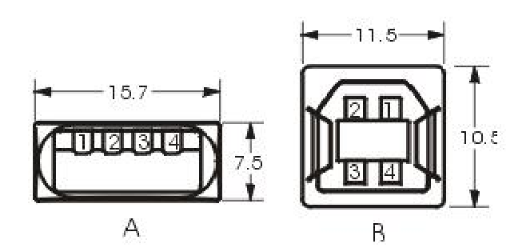
\includegraphics[scale=0.5]{res/img/usb_connector.png}
    \caption{Сечения разъемов USB кабеля. A – предназначены только для подключения к источнику, т.е. к компьютеру или хабу; В – предназначены только для подключения к периферийному устройству \cite{usb:specification}}
    \label{fig:usb_connector}
\end{figure}

\begin{table}[ht!]
  \caption{Назначение контактов и проводов USB кабеля \cite{usb:specification}}
    \centering
    \begin{tabular}{|c|c|c|}
    \hline
        \textbf{Номер контакта} & \textbf{Назначение} & \textbf{Цвет провода} \\ \hline
        \textbf{1} & V BUS & Красный \\ \hline
        \textbf{2} & D– & Белый \\ \hline
        \textbf{3} & D+ & Зеленый \\ \hline
        \textbf{4} & GND & Черный \\ \hline
        \textbf{Оплетка} & Экран & Оплетка \\ \hline
  \end{tabular}
  \label{tab:usb_signals}
\end{table}

\pagebreak

\section{Обзор протокола ULPI}

Современный рынок микросхем, поддерживающих обмен данными по шине USB, достаточно обширен, доступны продукты производства фирм Atmel, FTDI, Cypress, Intel, Microchip, National Semiconductor и др.

Для использования в работе была выбрана микросхема Microchip USB3300 по следующим причинам:

\begin{itemize}
\item полная поддержка протокола обмена по стандарту USB2.0;
\item возможность перепрограммирования номеров PID и VID, что позволяет избежать конфликтов при использовании микросхемы в различных устройствах;
\item возможность создания пользовательского устройства, без ограничений по выбору класса;
\item отсутствие накладных расходов на использование протокола, что позволяет полностью использовать пропускную способность USB2.0;
\item популярность и доступность микросхемы;
\item возможность использования стандартизированных UTMI+ блоков с минимальными доработками;
\item наличие документации как на саму микросхему, так и на все уровни протокола.
\end{itemize}

Микросхема USB3300 использует протокол UTMI+ Low Pin Interface (ULPI), позволяющий сократить количество интерфейсных линий, но требующий особого внимания к управлению шиной. В USB3300 протокол ULPI задействован как для настройки конфигурационных параметров приемопередатчика (таких как версия протокола и параметры кодирования), так и для приёма и передачи пакетов USB.

Назначения сигналов интерфейса описаны в таблице \ref{tab:ulpi_signals}.

  \begin{longtable}{|p{0.15\textwidth}|c|p{0.65\textwidth}|}
    \caption{Назначения сигналов интерфейса ULPI \cite{ulpi:usb3300, ulpi:specification}}
    \label{tab:ulpi_signals}
    \\ \hline
    \textbf{Сигнал} & \textbf{Направление} & \textbf{Описание} \\ \hline
    \endfirsthead
    \subcaption{Продолжение таблицы~\ref{tab:ulpi_signals}}
    \\ \hline \endhead
    \hline \subcaption{Продолжение на след. стр.}
    \endfoot
    \hline \endlastfoot
        \textbf{CLKOUT} & выход & \small{Интерфейсный тактовый генератор 60 МГц.} \\ \hline
        \textbf{\detokenize{DATA[7..0]}} & \detokenize{вход\выход} & \small{8-битная двунаправленная шина данных. Принадлежность шины определяется сигналом DIR. Контроллер и устройство инициируют передачу данных путем подачи ненулевого шаблона на шину данных. ULPI определяет синхронизацию интерфейса по нарастающему фронту CLKOUT. DATA\cite{lcd:display} - это старший разряд, а DATA[0] - младший. } \\ \hline
        \textbf{DIR} & выход & \small{Управляет направлением шины данных. DIR подтягивается к высокому уровню контроллером тогда, когда он не должен принимать данные от устройства.} \\ \hline
        \textbf{STP} & вход & \small{Устройство должно подавать сигнал STP, чтобы сигнализировать о завершении передачи пакета USB или операции записи в регистр, а также, по желанию, для остановки приема. Сигнал STP должен быть установлен после последнего байта данных.} \\ \hline
        \textbf{NXT} & выход & \small{Контроллер подает сигнал NXT для задержки отправки данных. Идентичен сигналам RxValid во время приема USB и TxReady во время передачи USB. Контроллер также одновременно подает сигналы NXT и DIR для индикации активности приема USB (RxActive), если до этого шина принадлежала устройству.}
  \end{longtable}

На рисунке \ref{fig:ulpi_dir_change} представлен пример изменения направления шины данных DATA. Каждое изменение владения шиной сопровождается циклом переключения, во время которого управление шиной данных неопределенно. Данные в таком цикле должны быть проигнорированы как контроллером, так и устройством \cite{ulpi:specification}.

\begin{figure}[ht]
    \centering
    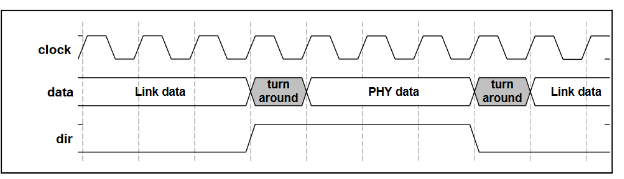
\includegraphics[scale=0.5]{res/img/ulpi_dir_change.png}
    \caption{Временная диаграмма изменения направления передачи данных \cite{ulpi:specification}}
    \label{fig:ulpi_dir_change}
\end{figure}

\begin{figure}[ht]
    \centering
    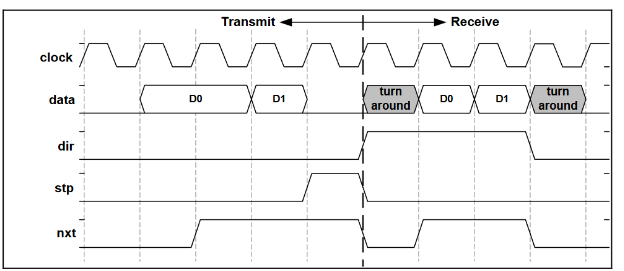
\includegraphics[scale=0.5]{res/img/ulpi_in_out.png}
    \caption{Временная диаграмма приёма и передачи данных \cite{ulpi:specification}}
    \label{fig:ulpi_in_out}
\end{figure}

На рисунке \ref{fig:ulpi_in_out} представлен пример приёма и передачи на шине ULPI: устройство, до этого владевшее шиной данных, устанавливает на шину ненулевые данные, тем самым начиная передачу. По завершении, оно устанавливает STP, указывая на конец передачи. Контроллер перехватывает управление шины, чтобы передать данные устройству. При этом, если больше новых данных нет, владение шиной вновь передаётся устройству \cite{ulpi:specification}.

\section{Интерфейс вывода изображения TTL}
Согласно спецификации дисплейного модуля ccb0702ih40ri-271c, предоставленной в качестве исходных данных для научно-исследовательской работы, его логика основана на интерфейсной микросхеме HX8264, спецификация которой приведена в рекомендуемом источнике \cite{lcd:driver} к заданию на исследовательскую работу. Однако доступ к её конфигурационным линиям не был распаян на шлейфе подключения. Это ограничивает возможности по управлению дисплеем.
Интерфейс передачи данных видеоизображения – TTL схож с протоколом VGA. Временная диаграмма и необходимые параметры задержки приведены на рисунках \ref{fig:ttl_timing} и \ref{fig:lcd_timing} соответственно.

\begin{figure}[ht]
    \centering
    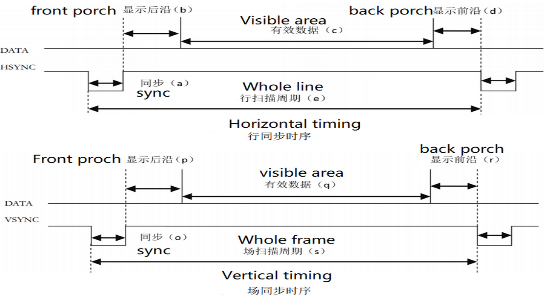
\includegraphics[scale=0.5]{res/img/ttl_timing.png}
    \caption{Временная диаграмма протокола TTL \cite{lcd:display}}
    \label{fig:ttl_timing}
\end{figure}

\begin{figure}[ht]
    \centering
    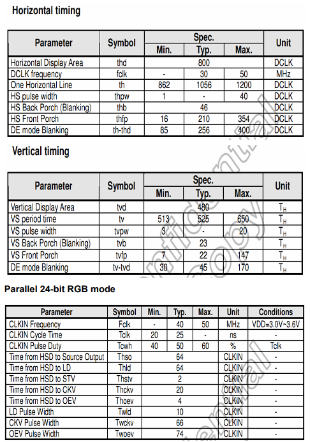
\includegraphics[scale=0.5]{res/img/lcd_timing.png}
    \caption{Временные характеристики матрицы \cite{lcd:display}}
    \label{fig:lcd_timing}
\end{figure}

\section{Кадровый буфер}

Для синхронизации работы устройства ULPI и видеовыхода необходим буфер, так как тактовые частоты и скорости передачи данных на этих шинах данных не совпадают. Буфер, содержащий кадр перед отправкой его на устройство видеовыхода, называется кадровым буфером.

В качестве кадрового буфера была выбрана память PSRAM, входящая в систему на кристалле ПЛИС Gowin GW1NR-9.

Модуль имеет достаточно простой интерфейс: шина адреса, шина данных и управляющие сигналы разрешения передачи данных и \detokenize{«data_mask»}, с помощью которго можно защитить часть данных от записи. В частности, сигнал «cmd» "--- это тип команды: 1 - запись, 0 - чтение. Сигнал \detokenize{«cmd_en»} обозначает момент начала ее выполнения. Все операции пакетные и длина пакета зависит от режима Burst Mode. Начинается пакет записываемых данных в один момент с началом команды. Операция записи в режиме Burst Mode - 16 показана на рисунке \ref{fig:psram_write}.

\begin{figure}[ht]
    \centering
    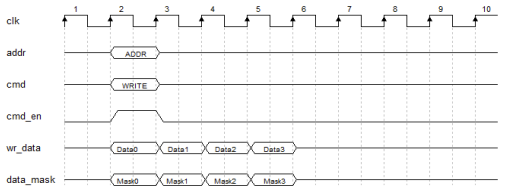
\includegraphics[scale=0.5]{res/img/psram_write.png}
    \caption{Временная диаграмма операции записи \cite{gowin:GW1NSR}}
    \label{fig:psram_write}
\end{figure}

\begin{figure}[ht]
    \centering
    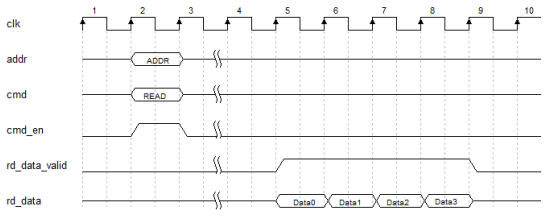
\includegraphics[scale=0.5]{res/img/psram_read.png}
    \caption{Временная диаграмма операции чтения \cite{gowin:GW1NSR}}
    \label{fig:psram_read}
\end{figure}

Операция чтения обозначена на рисунке \ref{fig:psram_read}. Читаемые данные появляются на шине не сразу, а через некоторое количество тактов. Это количество всегда постоянно и равно 16 тактам. Весь пакет данных из памяти сопровождается сигналом «\detokenize{rd_data_valid}».

\section{Выводы}

\begin{packed_enum}
\item Изучены рекомендуемые источники и выявлены другие источники.
\item Намечены разделы обзора и составлен (написан) сам обзор по теме НИР.
\item Обоснован выбор компонентной базы устройства отображения.
\item Описана работа кадрового буфера.
\item Представлены основные протоколы и интерфейсы устройств, используемых в данной работе.
\end{packed_enum}

\nocite{vhdl:specification}
